\documentclass[a4paper]{article}
\usepackage[top=1in, bottom=1.25in, left=1.25in, right=1.25in]{geometry}
\usepackage{amsmath}
\usepackage{multicol}
\usepackage{graphicx}
\usepackage[utf8]{inputenc}
\usepackage[english]{babel}
\setlength{\parskip}{0.03cm plus4mm minus3mm}
\RequirePackage{ltxcmds}[2010/12/07]

\usepackage{hyperref}
%opening
\title{Optical Hybrid}

\begin{document}

\maketitle

This block simulates a optical hybrid. It accepts two input signals corresponding to the signal and to the local oscillator. It generates four output signals. Figure ~\ref{opticalhybrid} shows a schematic representation of this block.

\begin{figure}[h]
	\centering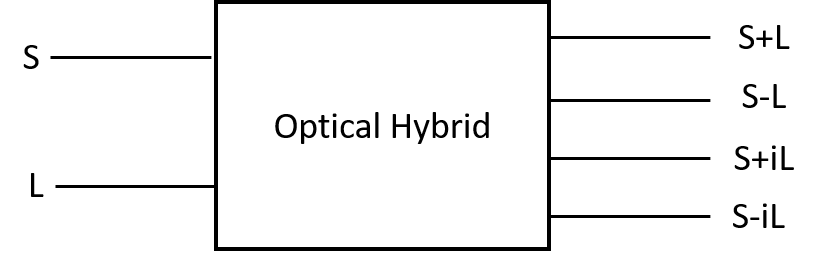
\includegraphics[width=0.6\textwidth]{optical_hybrid.png}
	\caption{Schematic representation of an optical hybrid}\label{opticalhybrid}
\end{figure}

\subsection*{Input Parameters}

\begin{itemize}
	\item opticalPower\{ 1e-3 \} 
	\item wavelength\{ 1550e-9 \}
	\item frequency\{ SPEED\_OF\_LIGHT / wavelength \}
\end{itemize}

\subsection*{Methods}
 
OpticalHybrid() {}
\bigbreak
OpticalHybrid(vector$<$Signal *$>$ \&InputSig, vector$<$Signal *$>$ \&OutputSig) :Block(InputSig, OutputSig) {}
\bigbreak
void initialize(void)
\bigbreak
bool runBlock(void)
\bigbreak
void setOutputOpticalPower(double outOpticalPower)
\bigbreak
void setOutputOpticalPower\_dBm(double outOpticalPower\_dBm)
\bigbreak
void setOutputOpticalWavelength(double outOpticalWavelength)
\bigbreak
void setOutputOpticalFrequency(double outOpticalFrequency) 

\subsection*{Functional description}

This block accepts two  input signals corresponding to the signal to be demodulated ($S$) and to the local oscillator ($L$). It generates four output optical signals given by $S+L$, $S-L$, $S+iL$, $S-iL$.

\pagebreak

\subsection*{Input Signals}

\subparagraph*{Number:} 2

\subparagraph*{Type:} Optical 

\subsection*{Output Signals}

\subparagraph*{Number:} 4

\subparagraph*{Type:} Optical 

\subsection*{Examples} 

\subsection*{Sugestions for future improvement}


\end{document}